\documentclass[12pt]{article}
\usepackage[utf8]{inputenc}
\usepackage[russian]{babel}
\usepackage{amsmath, amssymb}
\usepackage{graphicx}
\usepackage{float}
\usepackage{geometry}
\usepackage{listings}
\usepackage{xcolor}

\geometry{a4paper, left=2cm, right=2cm, top=2cm, bottom=2cm}

\lstset{
    language=Python,
    basicstyle=\small\ttfamily,
    keywordstyle=\color{blue},
    commentstyle=\color{green!50!black},
    stringstyle=\color{red},
    breaklines=true,
    showstringspaces=false,
    frame=single,
    numbers=left,
    numberstyle=\tiny\color{gray},
    captionpos=b
}



\begin{document}

\begin{titlepage}
    \begin{center}
        \vspace*{\fill}
        
        \textbf{\LARGE Лабораторная работа №3
«Интерполяционный кубический сплайн»}
        
        \vspace{0.5cm}
        
        \textbf{\Large  Николаева Ксения, 9 группа}
        
        
        \vfill
        
    \end{center}
\end{titlepage}

\tableofcontents
\newpage

\section{Постановка задачи}

На отрезке $[a, b]$ задана функция $f(x)$. Требуется вычислить значения функции в равноотстоящих узлах
$x_i = a + ih, i = 0, \ldots, N, h = (b-a)/N$ при $N = 15$. По полученной таблице $\{x_i, f(x_i)\}$ построить интерполяционный кубический сплайн $S_3(x)$ для функции $f(x)$ с дополнительными условиями, указанными в варианте задания.

В узлах $x_i = a + i \cdot \frac{b-a}{100}, i = 0, \ldots, 100$ вычислить значения сплайна $S_3(x)$ и сравнить со значениями функции $f(x)$ в этих узлах, т.е. найти $\max_{i=0,\ldots,100} |S_3(x_i) - f(x_i)|$. В одной системе координат построить график функции $f(x)$ и график интерполяционного кубического сплайна $S_3(x)$.

\subsection{Вариант 7}
Функция: $f(x) = x^2 \cos(2x), [a, b] = [-3, 3]$.

Дополнительные условия: $S''_3(a) = f''(a)$, $S''_3(b) = f''(b)$.

\section{Алгоритм построения интерполяционного кубического сплайна}

Пусть на отрезке $[a, b]$ задана функция $f(x)$ и разбиение $a = x_0 < x_1 < \ldots < x_N = b$. Кубический сплайн $S_3(x)$ представляет собой кусочно-заданную функцию, которая на каждом отрезке $[x_i, x_{i+1}]$ является многочленом третьей степени, а на всем отрезке $[a, b]$ обладает непрерывностью второго порядка.

Алгоритм построения интерполяционного кубического сплайна состоит из следующих шагов:

\begin{enumerate}
    \item На каждом отрезке $[x_i, x_{i+1}]$ сплайн представляется в виде:
    \begin{equation}
        S_3(x) = a_i + b_i(x-x_i) + c_i(x-x_i)^2 + d_i(x-x_i)^3
    \end{equation}
    где $i = 0, 1, \ldots, N-1$.
    
    \item Коэффициенты $a_i, b_i, c_i, d_i$ находятся из условий:
    \begin{itemize}
        \item Интерполяция: $S_3(x_i) = f(x_i)$ и $S_3(x_{i+1}) = f(x_{i+1})$ для $i = 0, 1, \ldots, N-1$.
        \item Непрерывность первой производной: $S'_3(x_i-0) = S'_3(x_i+0)$ для $i = 1, 2, \ldots, N-1$.
        \item Непрерывность второй производной: $S''_3(x_i-0) = S''_3(x_i+0)$ для $i = 1, 2, \ldots, N-1$.
    \end{itemize}

    \item Для определения всех коэффициентов требуются два дополнительных условия. В нашем варианте это:
    \begin{equation}
        S''_3(a) = f''(a), \quad S''_3(b) = f''(b)
    \end{equation}

    \item После подстановки условий получается система линейных уравнений относительно неизвестных коэффициентов сплайна, которая решается методом прогонки.
\end{enumerate}

\section{Построение интерполяционного кубического сплайна}

Для построения кубического сплайна в данной работе используется библиотека SciPy, функция CubicSpline, которая реализует описанный выше алгоритм. В качестве дополнительных условий задаются значения второй производной на концах отрезка.

Для функции $f(x) = x^2 \cos(2x)$ найдем вторую производную:
\begin{align}
f(x) &= x^2 \cos(2x) \\
f'(x) &= 2x\cos(2x) - 2x^2\sin(2x) \\
f''(x) &= 2\cos(2x) - 4x\sin(2x) - 4x\sin(2x) - 4x^2\cos(2x) \\
&= 2\cos(2x) - 8x\sin(2x) - 4x^2\cos(2x)
\end{align}

Таким образом, дополнительные условия:
\begin{align}
S''_3(-3) &= f''(-3) = 2\cos(-6) - 8(-3)\sin(-6) - 4(-3)^2\cos(-6) \\
&= 2\cos(6) + 24\sin(6) - 36\cos(6) \\
&\approx 2 \cdot 0.96 + 24 \cdot 0.28 - 36 \cdot 0.96 \\
&\approx 1.92 + 6.72 - 34.56 \\
&\approx -25.92
\end{align}

\begin{align}
S''_3(3) &= f''(3) = 2\cos(6) - 8(3)\sin(6) - 4(3)^2\cos(6) \\
&= 2\cos(6) - 24\sin(6) - 36\cos(6) \\
&\approx 2 \cdot 0.96 + 24 \cdot 0.28 - 36 \cdot 0.96 \\
&\approx 1.92 + 6.72 - 34.56 \\
&\approx -25.92
\end{align}

\section{Результаты}

\subsection{Максимальная погрешность}

По результатам вычислений получена максимальная погрешность:
\begin{equation}
    \max_{i=0,\ldots,100} |S_3(x_i) - f(x_i)| \approx 1.35853903 \times 10^{-2}
\end{equation}

\subsection{График функции и интерполяционного кубического сплайна}

\begin{figure}[H]
    \centering
    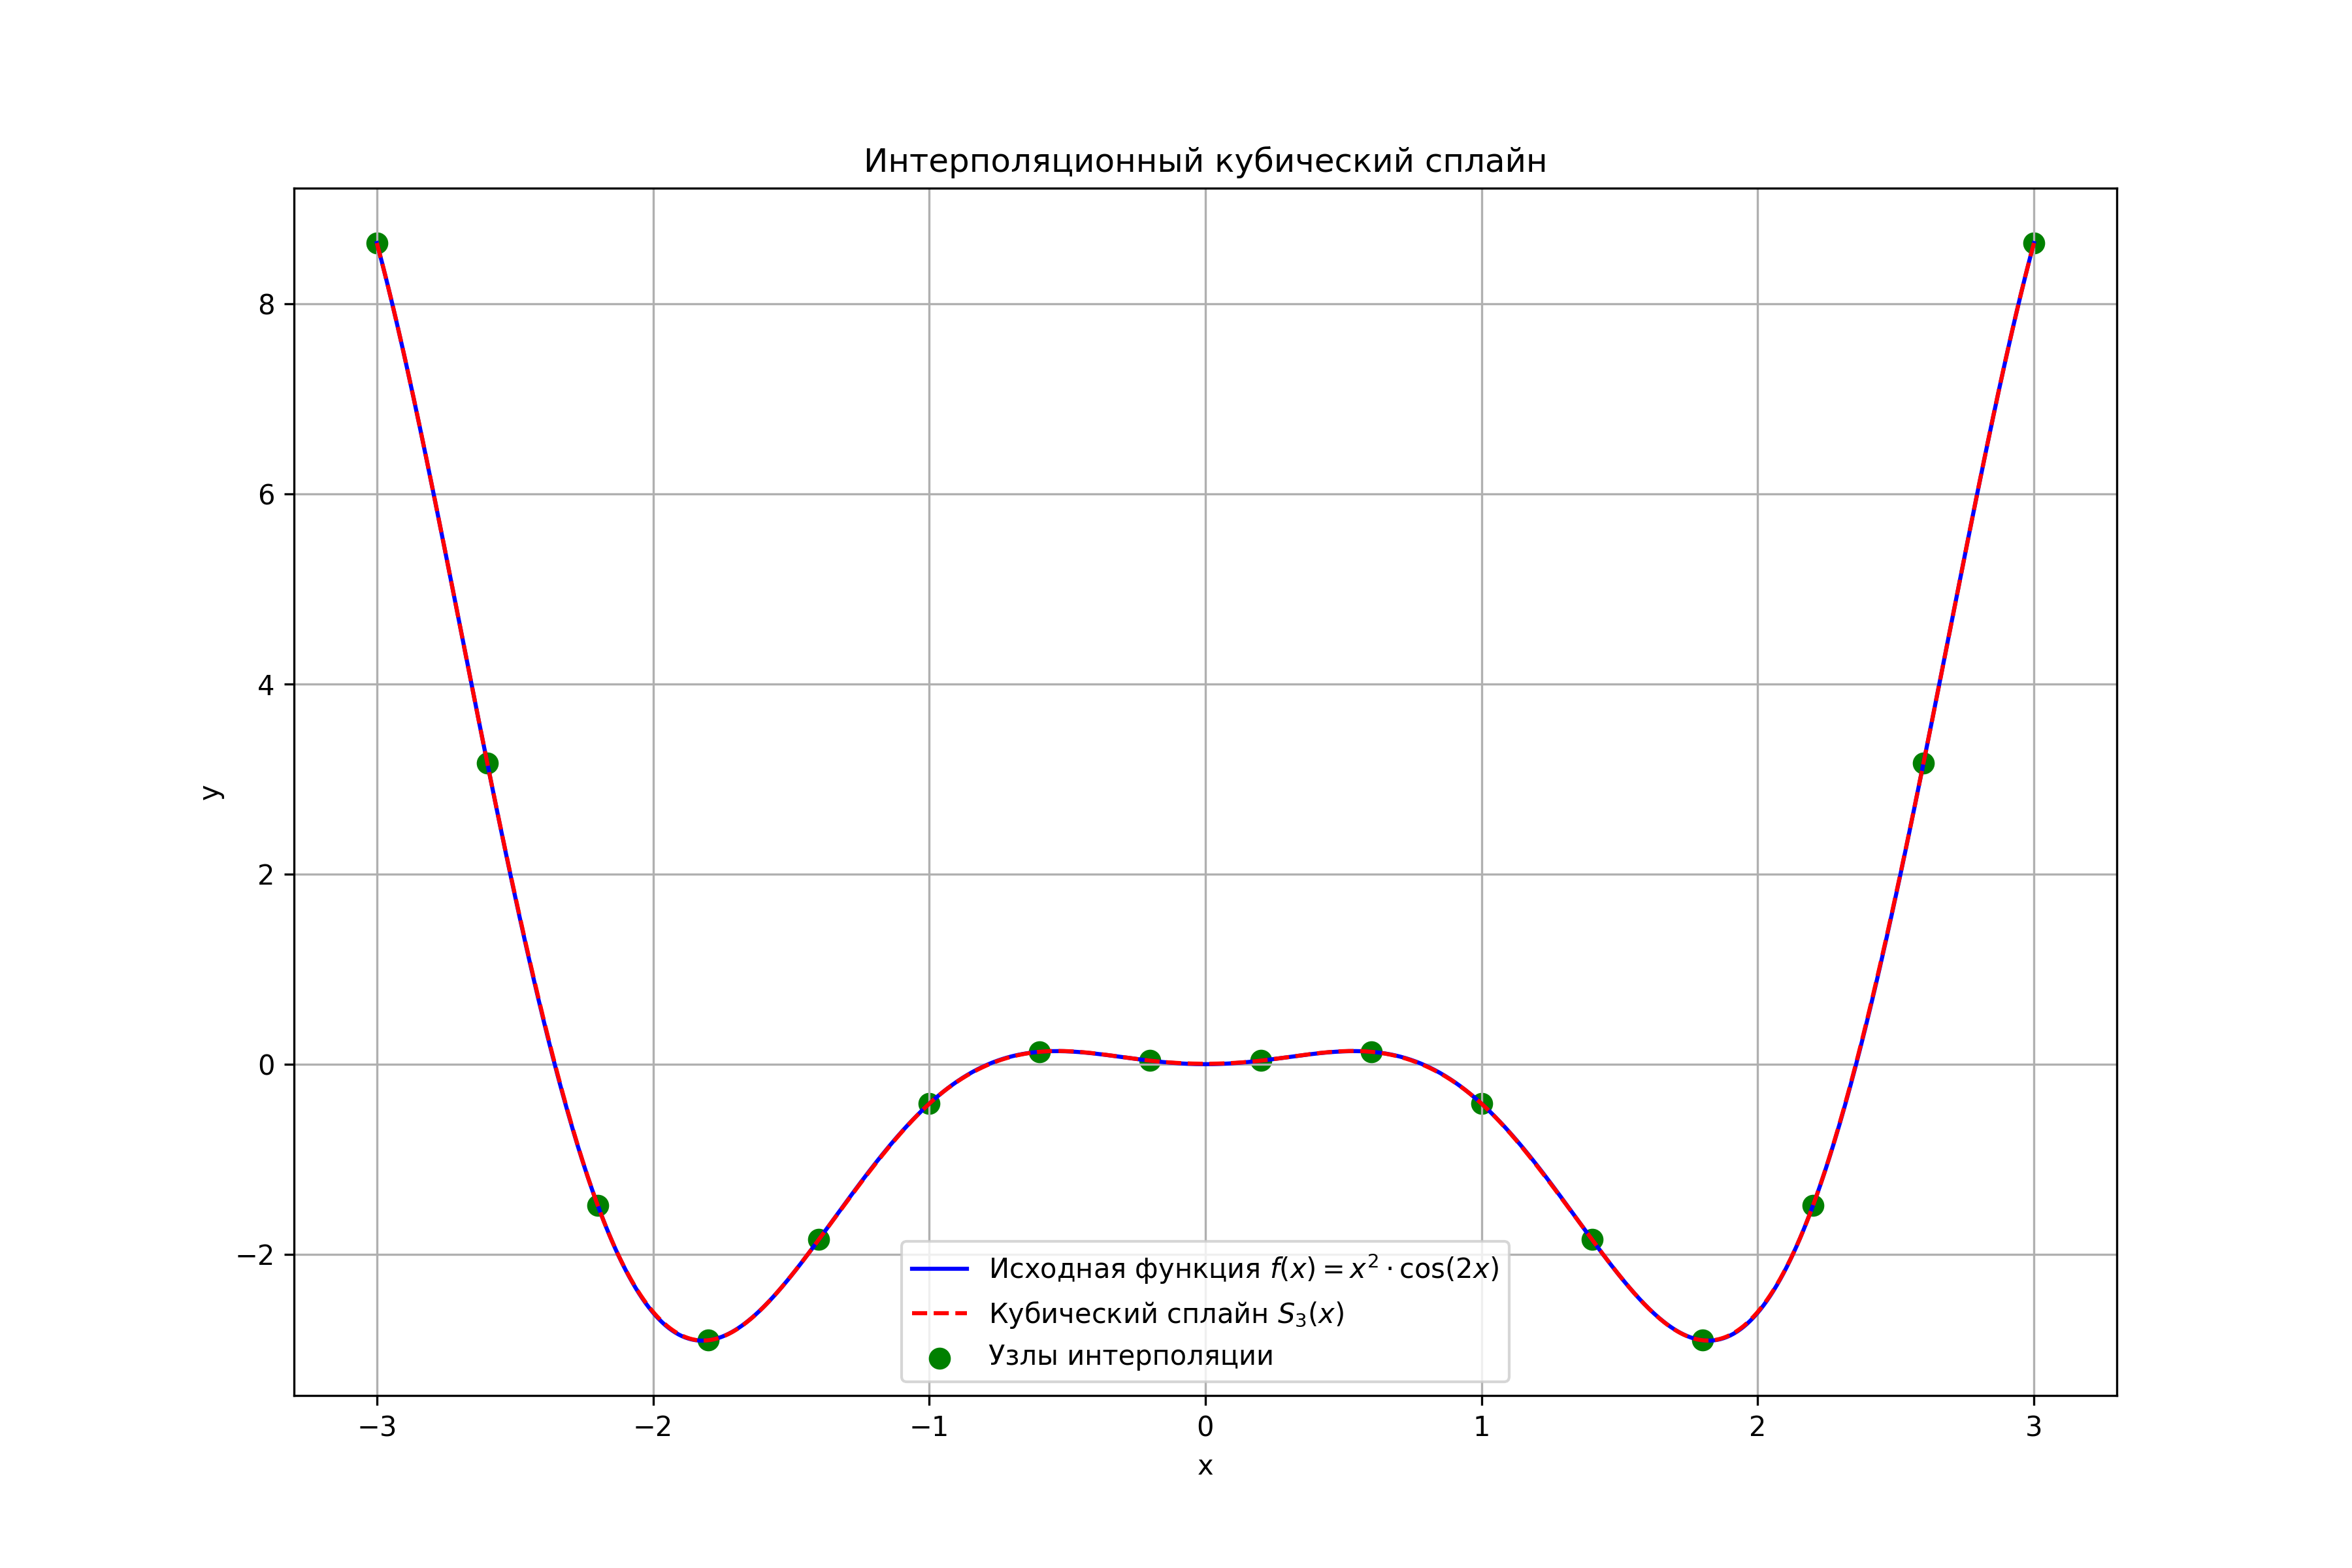
\includegraphics[width=0.9\textwidth]{spline_plot.png}
    \caption{График функции $f(x) = x^2\cos(2x)$ и интерполяционного кубического сплайна $S_3(x)$}
    \label{fig:spline}
\end{figure}

\section{Выводы}

В данной лабораторной работе был построен интерполяционный кубический сплайн для функции $f(x) = x^2\cos(2x)$ на отрезке $[-3, 3]$ с дополнительными условиями $S''_3(-3) = f''(-3)$ и $S''_3(3) = f''(3)$.

Полученные результаты показывают:
\begin{itemize}
    \item Кубический сплайн $S_3(x)$ хорошо аппроксимирует исходную функцию $f(x)$ на всем отрезке $[-3, 3]$.
    \item Максимальная погрешность интерполяции составляет примерно $1.35853903 \times 10^{-2}$, что говорит о высокой точности интерполяции.
    \item Дополнительные условия на вторые производные на концах отрезка обеспечивают хорошее поведение сплайна вблизи границ, особенно в точках с более сложным поведением функции.
    \item Визуально графики функции и сплайна практически совпадают, что подтверждает эффективность кубической сплайн-интерполяции для данного класса функций.
\end{itemize}

В качестве наблюдения можно отметить, что метод кубической сплайн-интерполяции особенно эффективен для функций, которые имеют осциллирующее поведение (как в нашем случае $f(x) = x^2\cos(2x)$), поскольку сплайн хорошо приближает функцию даже при относительно небольшом количестве узлов ($N = 15$).

При увеличении числа узлов интерполяции $N$ точность аппроксимации будет возрастать. Метод кубических сплайнов превосходит полиномиальную интерполяцию Лагранжа или Ньютона при работе с большим количеством узлов, поскольку не подвержен эффекту Рунге.

\section{Листинг программы}

\begin{verbatim}
    import numpy as np
import matplotlib.pyplot as plt

# Определение функции и её второй производной
def f(x):
    """
    Функция: f(x) = x^2 * cos(2x)
    """
    return x**2 * np.cos(2*x)

def f_second_derivative(x):
    """
    Вторая производная функции f(x) = x^2 * cos(2x)
    f''(x) = 2*cos(2*x) - 8*x*sin(2*x) - 4*x^2*cos(2*x)
    """
    return 2*np.cos(2*x) - 8*x*np.sin(2*x) - 4*x**2*np.cos(2*x)

def tridiagonal_solve(a, b, c, d):
    """
    Решение трехдиагональной системы методом прогонки
    
    a[i]*x[i-1] + b[i]*x[i] + c[i]*x[i+1] = d[i], i = 0,1,...,n-1
    
    Параметры:
    a - диагональ под главной (начинается с a[1])
    b - главная диагональ
    c - диагональ над главной (заканчивается c[n-2])
    d - правая часть
    
    Возвращает:
    x - решение системы
    """
    n = len(d)
    alpha = np.zeros(n)
    beta = np.zeros(n)
    x = np.zeros(n)
    
    # Прямой ход
    alpha[0] = -c[0] / b[0]
    beta[0] = d[0] / b[0]
    
    for i in range(1, n-1):
        denom = b[i] + a[i] * alpha[i-1]
        alpha[i] = -c[i] / denom
        beta[i] = (d[i] - a[i] * beta[i-1]) / denom
    
    # Последний элемент
    x[n-1] = (d[n-1] - a[n-1] * beta[n-2]) / (b[n-1] + a[n-1] * alpha[n-2])
    
    # Обратный ход
    for i in range(n-2, -1, -1):
        x[i] = alpha[i] * x[i+1] + beta[i]
    
    return x

def build_cubic_spline(x_nodes, y_nodes):
    """
    Построение кубического сплайна методом прогонки с граничными условиями: 
    S''(a) = f''(a), S''(b) = f''(b)
    
    Параметры:
    x_nodes - узлы интерполяции
    y_nodes - значения функции в узлах
    
    Возвращает:
    coefficients - коэффициенты сплайна (a, b, c, d) для каждого участка
    """
    n = len(x_nodes) - 1  # Количество участков
    
    # Шаги между узлами
    h = np.diff(x_nodes)
    
    # Правые части уравнений (разности разделенных разностей)
    F = np.zeros(n+1)
    for i in range(1, n):
        F[i] = 6 * ((y_nodes[i+1] - y_nodes[i]) / h[i] - (y_nodes[i] - y_nodes[i-1]) / h[i-1]) / (h[i] + h[i-1])
    
    # Граничные условия: значения второй производной на концах
    F[0] = f_second_derivative(x_nodes[0])  # S''(a) = f''(a)
    F[n] = f_second_derivative(x_nodes[n])  # S''(b) = f''(b)
    
    # Формирование коэффициентов трехдиагональной матрицы
    a = np.zeros(n+1)  # Диагональ под главной
    b = np.zeros(n+1)  # Главная диагональ
    c = np.zeros(n+1)  # Диагональ над главной
    
    # Заполнение коэффициентов для граничных условий
    b[0] = 1.0
    c[0] = 0.0
    a[n] = 0.0
    b[n] = 1.0
    
    # Заполнение коэффициентов для внутренних узлов
    for i in range(1, n):
        a[i] = h[i-1] / (h[i-1] + h[i])
        b[i] = 2.0
        c[i] = h[i] / (h[i-1] + h[i])
    
    # Решение системы методом прогонки для получения m[i] = S''(x[i])
    m = tridiagonal_solve(a, b, c, F)
    
    # Вычисление коэффициентов сплайна для каждого участка
    coefficients = []
    for i in range(n):
        # Коэффициенты для i-го участка [x[i], x[i+1]]
        a_i = y_nodes[i]
        b_i = (y_nodes[i+1] - y_nodes[i]) / h[i] - h[i] * (m[i+1] + 2 * m[i]) / 6
        c_i = m[i] / 2
        d_i = (m[i+1] - m[i]) / (6 * h[i])
        
        coefficients.append((a_i, b_i, c_i, d_i))
    
    return coefficients, x_nodes

def evaluate_spline(x, coefficients, x_nodes):
    """
    Вычисление значения сплайна в точке x
    
    Параметры:
    x - точка для вычисления
    coefficients - коэффициенты сплайна
    x_nodes - узлы интерполяции
    
    Возвращает:
    y - значение сплайна в точке x
    """
    if x < x_nodes[0] or x > x_nodes[-1]:
        raise ValueError("x лежит вне диапазона узлов интерполяции")
    
    # Поиск участка, которому принадлежит x
    i = 0
    while i < len(x_nodes) - 1 and x > x_nodes[i+1]:
        i += 1
    
    # Использование коэффициентов для данного участка
    a_i, b_i, c_i, d_i = coefficients[i]
    dx = x - x_nodes[i]
    
    # Вычисление значения сплайна
    y = a_i + b_i * dx + c_i * dx**2 + d_i * dx**3
    
    return y

def evaluate_spline_array(x_array, coefficients, x_nodes):
    """
    Вычисление значений сплайна для массива точек
    """
    y_array = np.zeros_like(x_array)
    for i, x in enumerate(x_array):
        y_array[i] = evaluate_spline(x, coefficients, x_nodes)
    return y_array

def main():
    """
    Основная функция для решения задачи
    """
    # Параметры задания
    a, b = -3, 3  # Границы отрезка [a, b]
    N = 15  # Количество интервалов
    
    # 1. Вычисление значений функции в равноотстоящих узлах
    h = (b - a) / N
    x_nodes = np.array([a + i * h for i in range(N + 1)])
    y_nodes = f(x_nodes)
    
    # 2. Построение интерполяционного кубического сплайна
    spline_coeffs, x_spline = build_cubic_spline(x_nodes, y_nodes)
    
    # 3. Вычисление значений сплайна и исходной функции в узлах для сравнения
    n_test = 101  # 101 точка для i = 0, 1, 2, ..., 100
    x_test = np.array([a + i * (b - a) / 100 for i in range(n_test)])
    y_true = f(x_test)
    y_spline = evaluate_spline_array(x_test, spline_coeffs, x_nodes)
    
    # 4. Вычисление максимальной погрешности
    errors = np.abs(y_spline - y_true)
    max_error = np.max(errors)
    max_error_idx = np.argmax(errors)
    
    # 5. Вывод результатов
    print(f"Максимальная погрешность: {max_error:.8e}")
    print(f"Достигается в точке x = {x_test[max_error_idx]:.4f}")
    
    # 6. Построение графиков
    plt.figure(figsize=(12, 8))
    
    # График исходной функции
    x_plot = np.linspace(a, b, 1000)
    plt.plot(x_plot, f(x_plot), 'b-', label='Исходная функция $f(x) = x^2 \cdot \cos(2x)$')
    
    # График сплайна
    y_spline_plot = evaluate_spline_array(x_plot, spline_coeffs, x_nodes)
    plt.plot(x_plot, y_spline_plot, 'r--', label='Кубический сплайн $S_3(x)$')
    
    # Узлы интерполяции
    plt.scatter(x_nodes, y_nodes, color='green', s=50, label='Узлы интерполяции')
    
    plt.grid(True)
    plt.legend()
    plt.title('Интерполяционный кубический сплайн (метод прогонки)')
    plt.xlabel('x')
    plt.ylabel('y')
    
    # Вывод графика
    plt.savefig('spline_plot_custom.png', dpi=300)
    plt.show()
    
    # Вычисление значений второй производной функции в граничных точках
    print(f"\nЗначение f''({a}) = {f_second_derivative(a):.6f}")
    print(f"Значение f''({b}) = {f_second_derivative(b):.6f}")
    
    # 7. Вывод таблицы сравнения значений в узлах
    print("\nТаблица сравнения значений в узлах интерполяции:")
    print("{:<10} {:<15} {:<15} {:<15}".format("i", "x_i", "f(x_i)", "S_3(x_i)"))
    print("-" * 55)
    
    y_spline_nodes = evaluate_spline_array(x_nodes, spline_coeffs, x_nodes)
    for i, (x, y_true_val, y_spline_val) in enumerate(zip(x_nodes, y_nodes, y_spline_nodes)):
        print("{:<10} {:<15.6f} {:<15.6f} {:<15.6f}".format(i, x, y_true_val, y_spline_val))
    
    return spline_coeffs, x_nodes, y_nodes, max_error

if __name__ == "__main__":
    spline_coeffs, x_nodes, y_nodes, max_error = main()
    
    # Отображаем максимальную погрешность для отчета
    print(f"\nЗначение max |S_3(x_i) - f(x_i)| = {max_error:.8e}")
    
    # Дополнительно: вывод аналитического выражения для f''(x)
    print("\nАналитическое выражение для f''(x):")
    print("f''(x) = 2*cos(2*x) - 8*x*sin(2*x) - 4*x^2*cos(2*x)")
\end{verbatim}

\end{document}